% Plantilla realizada por Santiago Morante Cendrero
% Tuneada por Javi

%parametros de tipo libro
\documentclass[10pt,a4paper]{book}

%idioma espa�ol y acentos
\usepackage[spanish]{babel}
\usepackage[latin1]{inputenc}

%algunos s�mbolos matem�ticos y paquete para usar subim�genes
\usepackage{amsmath}
\usepackage{amsfonts}
\usepackage{amssymb}
\usepackage{graphicx}
\usepackage{subfigure}
\usepackage{listings}
\usepackage{appendix}

%para generar �ndice con hiperv�nculos
\usepackage{hyperref}

%parametros del documento (sus propiedades)
\hypersetup{
    pdftitle={Nombre del alumno - TFG - a�o},
    pdfsubject={TFG - a�o},
    pdfauthor={Nombre del alumno},
    pdfkeywords={palabraclave1} {palabraclave2} {palabraclave3},
    colorlinks,
    citecolor=black,
    filecolor=black,
    linkcolor=black,
    urlcolor=black,
}

%empieza el documento
\begin{document}  

%elementos antes del trabajo en s� se meten dentro de frontmatter
\frontmatter

%cada incluye referencia a un archivo de tipo .tex
\begin{titlepage}
\begin{center}

%forma de introducir im�genes. el \\[0.5 cm] de final de l�nea introduce un salto de ese tama�o.
%width=1\textwidth indica el tama�o de la im�gen (valores entre 0-1). 
 
\includegraphics[width=1\textwidth]{figuras/cabecera.png}  \\[0.5 cm]

\large \textsc{Departamento de Ingenier�a...} \\ [1 cm]

\large TRABAJO FIN DE GRADO\\[1 cm]

\huge \textsc{T�tulo del trabajo}\\[7 cm]

%flushleft alinea a la izquierda el texto
\begin{flushleft} \Large
\emph{Autor:} nombre del alumno\\[0.5 cm]
\emph{Director:} nombre del director \\
\emph{Tutor:} nombre del tutor
\end{flushleft}

%rellena de blanco el resto de la p�gina para escribir abajo del todo
\vfill

% Bottom of the page
{\large Ciudad, Mes a�o}

\end{center}
\end{titlepage}

\begin{flushleft}

Copyright \copyright  2014. Javier Isabel Hern�ndez

Esta obra est� sujeta a la licencia Reconocimiento-NoComercial-CompartirIgual 4.0 Internacional de Creative Commons. Para ver una copia de esta licencia, visite http://creativecommons.org/licenses/by-nc-sa/4.0/.


\end{flushleft}

\cleardoublepage

\begin{flushleft} \large
\textbf{T�tulo:} TODO \\
\textbf{Autor:} Javier Isabel Hern�ndez\\
\textbf{Director:} F�lix Rodr�guez Ca�adillas \\ 
\textbf{Tutor:} Alberto Jard�n Huete\\ [1 cm]

\end{flushleft} 

\begin{center} \LARGE
EL TRIBUNAL \\ [1 cm]
\end{center}

\begin{flushleft} \LARGE
Presidente: \\ [1 cm]
Vocal: \\ [1 cm]
Secretario: \\ [1.5 cm]
\end{flushleft}

\large
Realizado el acto de defensa y lectura del Trabajo Fin de Grado el d�a ....... de ....................   de ... en .........., en la Escuela Polit�cnica Superior de la Universidad Carlos III de Madrid, acuerda otorgarle la CALIFICACI�N de: \\ [2 cm]

\begin{center}
 \large VOCAL \\ [2.2 cm]
\end{center}

\begin{minipage}{0.5\textwidth}
 \begin{flushleft}
 \large SECRETARIO
\end{flushleft}
\end{minipage}
\begin{minipage}{0.5\textwidth}
\begin{flushright}
 \large PRESIDENTE
\end{flushright} 
\end{minipage}

\chapter{Agradecimientos}

En primer lugar me gustar�a agradecer a mi tutor, Alberto Jard�n, y a mi director F�lix Rodr�guez, el haberme dado la oportunidad de realizar un trabajo de final de grado que me apasiona.

Quiero dar las gracias a Miguel Gonz�lez-Fierro, por darme tan buenos consejos TODO



Quiero dar las las gracias de todo coraz�n a mi familia, a mi padre Javier, a mi madre Miriam y a mi hermana Marta. A ellos que siempre me han apoyado en todas las decisiones que he dedicido tomar, me han animado a perseguir mis objetivos y me han consolado en los momentos mas dif�ciles.

Por �timo, quiero dar las gracias a mi novia Silvia, que ha estado a mi lado anim�ndome siempre que lo he necesitado, y a quien he prometido que llevar� a la playa en cuanto termine este proyecto. 




%chapter introduce un nuevo cap�tulo
\chapter{Resumen}




En este proyecto se ha desarrollado la plataforma rob�tica mini-humanoide Raider, (Robot Antropom�rfico para la Investigaci�n y Desarrollo en Entornos Reales) con capacidad para actuar de forma aut�noma bas�ndose en algoritmos de visi�n por computador. Para ello se ha dise�ado una configuraci

 integrado en el robot mini-humanoide un sistema de procesamiento de im�genes formado por una c�mara USB y un controlador desarrollado sobre un ordenador de tama�o reducido, As� como diferentes sensores que apoyen a la parte de vision.( TODO mejorar el t�rmino )
Tras dise�ar, fabricar y montar las nuevas piezas se ha procedido a programar el robot. En la programaci�n de la locomoci�n se presentan los pasos que se han seguido desde el movimiento de una articulaci�n simple hasta la combinacion de estos movimientos para producir movimientos mas complejos como la caminata o el control del equilibrio. Por otra parte, se han estudiado y desarrollado algoritmos de visi�n en los que el robot basar� su comportamiento. Mas espec�ficamente, se han desarrollado t�cnicas de path planning basadas en la b�squeda de trayectorias mediante la detecci�n y esquelitizaci�n del espacio navegable basada en el algoritmo de de ZANG SHUEN. Adicionalmente, se han programado otras funciones como el tracking de una pelota o la lectura de c�digos qr.

El procesamiento de im�genes se ha combinado con la informaci�n recibida por los sensores para dise�ar aplicaciones aptas para la competici�n en CEABOT y otros eventos. Para concluir el proyecto, el robot se ha presentado a la edici�n de 2014 de CEABOT.

El proyecto queda como una plataforma viable sobre la que realizar nuevos proyectos por sus capacidades y robustez.



\paragraph{Palabras clave:} palabraclave1, palabraclave2, palabraclave3.

\chapter{Abstract}

(El resumen en ingles)

\paragraph{Keywords:} keyword1, keyword2, keyword3.

%genera �ndice
\tableofcontents

%�ndice de figuras. Tambi�n se podr�a hacer uno de tablas (listoftables)
\listoffigures
 
%empieza la parte descriptiva del trabajo
\mainmatter
 
\chapter{Introducci�n}

En este cap�tulo...

%section es un apartado dentro de un chapter. Tambi�n existe subsection y subsubsection

%las referencias a art�culos se ponen con \cite, 
%las referencias a im�genes \ref, 
%y las referencias a ecuaciones \eqref

Este tema.... Esto es un ejemplo de cita de un art�culo \cite{gonzalezeducational}.

%itemize es una lista. Cada t�rmino lleva delante un \item
\begin{itemize}
\item \textbf{ejemplo de lista de puntos}. Ejemplo.
\item \textbf{ejemplo2 de lista}. Ejemplo2.
\end{itemize} 

Ejemplo de referencia a figura (figura \ref{uc3m}).

%caption es el pie de foto, y label es el nombre que se da a la imagen para referenciarla despu�s. label no puede llevar acentos y no se muestra de cara al documento final (es s�lo interno).
\begin{figure}[h]
\centering

\includegraphics[width=0.45\textwidth]{figuras/uc3m}   
\caption{Logotipo de la UC3M \copyright UC3M}
\label{uc3m}
\end{figure}



La idea...

\section{Introduccion a la rob�tica Open-Source TODO}

TODO TODO TODO TODO TODO (Lo siguiente son ideas sueltas sin orden)

En los ultimos a�os blablabla impresoras 3d. El uso de esta nueva herramienta ha revolucionado blablabla hacer robots. La fabricaci�n de piezas, que en la mayor�a de los caso resultaba inaccesible para los estudiantes interesados en construir sus propios prototipos, se ha visto impulsada enormemente. Gracias a esto ahora tenemos a nuestro alcance la posibilidad de fabricar de una forma muy r�pida y econ�mica robots de un nivel superior al que estamos acostumbrados a ver.

Una de las ramas de la rob�tica que mas puede haberse beneficiado de este hecho es la rob�tica humanoide. 

El campo de la rob�tica humanoide tiene como objetivo el desarrollo de robots antropom�rficos. El motivo principal es favorecer el hecho de que los robots se desenvuelvan en entornos dise�ados por y para seres humanos. Otros robots, como los robots m�viles movidos por ruedas, suelen necesitar entornos modificados convenientemente para poder suplir las necesidades que se requieren. Por el contrario, un robot humanoide posee la ventaja de poder interaccionar con un entorno ya existente, as� como la posibilidad de utilizar herramientas humanas. Por supuesto, el acceso de un alumno a un robot de este tipo parece algo impensable. Es por ello que en la asociaci�n de rob�tica existe un linea de investigaci�n de mini-humanoides. A priori, puede parecer que este tipo de robots est�n muy alejados de los humanoides de los laboratorios mas famosos, sin embargo, suponen un punto de partida viable para el comienzo de su estudio. Los miembros del grupo de mini-humanoides, tienen la oportunidad de trabajar libremente con robots reales, experimentando con su construcci�n, programaci�n y modificaci�n.


 Acostumbrados a verla como una linea de investigaci�n inaccesible . blablabla es cara y practicamente la �nica forma que tiene un estudiante de darle ca�a es con simulaciones.

Si bien es cierto, esto no significa que los robots imprimibles vayan a sustituir a los robots caros de laboratorio, pero suponen una primera aproximaci�n a ellos.

TODO TODO Esto hay que ver si se hila con el siguiente apartado o se separa

\section{Asociaci�n de Rob�tica de la Universidad Carlos III}

La Asociaci�n de Rob�tica de la Universidad Carlos III de Madrid, AsRob, surgi� en el a�o 2006 con el objetivo de acercar la rob�tica a los alumnos de la universidad que compart�an inquietudes e inter�s por el campo de la rob�tica.

A d�a de hoy, la asociaci�n cuenta con mas de cien ( <- TODO cuantos ) miembros activos repartidos en cinco lineas de investigaci�n independientes, como son:
\begin{itemize}
\item \textbf{Veh�culos A�reos no Tripulados (UAVs)}.
\item \textbf{Robot Devastation}.
\item \textbf{Robots Personales de Competici�n}.
\item \textbf{Robots Mini-Humanoides}.
\item \textbf{Impresoras 3D Open-Source}.
\end{itemize}

Sin embargo, cabe destacar que aunque se trata de proyectos diferentes, existe una gran sinergia entre ellos. Particularmente, los miembros de la linea de Robots Mini-Humanoides, estamos muy ligados al estudio de las impresoras 3D, investigando diferentes t�cnicas de impresi�n, dise�o de estructuras y materiales. Ejemplo de ello es el proyecto MYOD ( <- TODO referencia ), en el que se propone la construcci�n de robots mini-humanoides compuestos integramente con piezas impresas y replicables.


\section{Descripci�n del proyecto TODO}

blablablabla mi proyecto es la monda

\section{Estructura del documento TODO}

A continuaci�n y para facilitar la lectura del documento, se detalla el contenido de cada cap�tulo.

\begin{itemize}
\item En el cap�tulo 1 se realiza una introducci�n.
\item En el cap�tulo 2 se hace un repaso...
\end{itemize}


%chapter introduce un nuevo cap�tulo

\chapter{Objetivos TODO ESQUEMATIZADO }

%gmmgfngfngfngfngfngfnhgf
%\begin{itemize}
%\item \textbf{ejemplo de lista de puntos}.

%Cocoloco loco loco loco tacacacaca
%\item \textbf{ejemplo de lista de puntos}.\\Cocoloco loco loco loco %tacacacaca
%\item \textbf{ejemplo2 de lista}.
%\end{itemize}

\section{Desarrollar una plataforma rob�tica humanoide}

TODO El primer objetivo de este proyecto es el desarrollo de una plataforma rob�tica humanoide de prop�sito general. Para llegar a ello ser� necesario estudiar los componentes que forman un robot humanoide Sus capacidades deben ser al menos suficientes para desarrolar sobre la plataforma los objetivos del segundo punto.

- Que la plataforma sea lo suficientemente cojonuda para poder hacer esto y mas 

\subsection{Estudiar los componentes que necesita un robot humanoide}

- Se realizar� un estudio de elementos necesarios para un robot
- Se evaluar� cuales funcionan mejor y peor
- Se analizar� cuales son dignos de meterse en mi robot
- Se escoger� una configuraci�n completa 

\subsection{Integrar una c�mara USB}

- Se requiere integrar una c�mara para hacer algoritmos de visi�n
- Se requiere que la c�mara entre integrada f�sicamente en el robot.
- Que la c�mara pueda moverse en el robot.

\subsection{Integrar un controlador}

- Un controlador que permita mover el robot y procesar visi�n.
- Que pueda programarse libremente sin casarse con Robotis.
- Que permita a�adir sensores y actuadores libremente.
- Que se integre fisicamente dentro del robot.
- Que funcione (capacidades de procesamiento, autonom�a... etc)


\subsection{Realizar las modificaciones esctructurales que sean pertinentes}

- Dise�ar piezas que requiera el robot (para montar sensores, c�mara...)
- Dise�ar piezas que no se requieran pero mejoren el comportamiento
- Dise�arlas para que puedan imprimirse con una impresora 3d.
- Imprimirlas todas

\section{Puesta en marcha y programaci�n}

El robot debe ponerse en marcha y funcionar, desde su montaje hasta su participaci�n en CEABOT

\subsection{Desarrollar locomoci�n}

- Controlar movimientos de las articulaciones
- Programar movimientos complejos
- Hacer que ande
Hacer el control de movimientos desde el movimiento de un servo has el movimiento de extremidades y con ello 

\subsection{Desarrollar algoritmos de visi�n}

- Hacer algoritmos de visi�n con OpenCV
- Que funcionen dentro del robot
- Optimizados para funcionar en condiciones



\subsection{Desarrollar aplicaciones de competici�n}

- Apoyandose en vision
- Con los movimientos creados
- Integrando la informaci�n de sensores
- Consiguiendo pasar las pruebas

sando de base las dos cosas anteriores el robot tiene que poder funcionar los suficientemente bien como para hacer programillas para las pruebas concretas.





\paragraph{Palabras clave:} TODO palabraclave1, palabraclave2, palabraclave3.


%chapter introduce un nuevo cap�tulo
\chapter{Descripci�n de la linea de investigaci�n}

TODO

\paragraph{Palabras clave:} palabraclave1, palabraclave2, palabraclave3.
 %Descripcion de la linea de investigacion

\chapter{Estado del arte}



\section{Plataformas rob�ticas mini-humanoides}

Robots 



\section{Competiciones}
\subsection{RoboGames}

Robots estructuralmente molones multidisciplinares


\subsection{Robo-One}

Robots estructuralmente molones, fuertes, estables, radiocontrolados. Compiten cara a cara muchos equipos

\subsection{Robocup}

Enjambres, vision, proramaci�n coordinada. Entornos din�micamente VARIABLES.

\subsection{Ceabot}

Robots individuales, compiten solos en entornos "complejos" pero FIJOS

\section{Locomoci�n}
hablar del motion, del pypose... contra un zmp y cosas asi



\section{Visi�n}


 %Estado del arte

%chapter introduce un nuevo cap�tulo
\chapter{Descripci�n de las herramientas a utilizar}

\section{Herramientas de dise�o y fabricaci�n de piezas}
\subsection{OpenSCAD}
\subsection{Impresi�n 3d}
\section{Herramientas de dise�o de circuitos}
\subsection{KiCad}

\section{Herramientas de programaci�n}
\subsection{Qt Creator}
\subsection{CM9 IDE}
\subsection{CMake}


CM9 IDE es un entorno de programaci�n basado en Arduino IDE, preparada para programar placas electr�nicas de la serie OpenCM.



\subsection{OpenCV}

\paragraph{Palabras clave:} palabraclave1, palabraclave2, palabraclave3.
 %Descripcion de las herramientas a utilizar
  
\chapter{Desarrollo y montaje}\label{chaptermontaje}

En este cap�tulo se mostrar�n los procedimientos que se han seguido para montar algunos componentes. Hasta este punto hemos definido una colecci�n de sensores, actuadores y piezas; el siguiente paso ser� integrar y conectarlos todos en el robot.

\section{Adecuaci�n de sensores}

Los sensores utilizados, tal y como se detall� en la selecci�n de componentes, ser�n: un aceler�metro y giroscopio MPU9150, una br�jula CMPS03 y dos infrarrojos Sharp. A continuaci�n se muestra c�mo han sido conectados al controlador principal, la BeagleBone Black. 

\subsection{Infrarrojos Sharp}

Los sensores infrarrojos modelo GP2Y0A21YK0F de la marca Sharp, permiten variar la tensi�n de alimentaci�n entre -0.3 y 7V, pero experimentalmente se ha observado que la mayor precisi�n se alcanza a 5V. A esta tensi�n, podemos observar en la hoja de caracter�sticas\cite{cooperationgp2y0a02yk} del sensor la gr�fica \ref{graficair}, en la que se muestra el valor de la salida del sensor respecto a la distancia medida.

\begin{figure}[H]
\centering
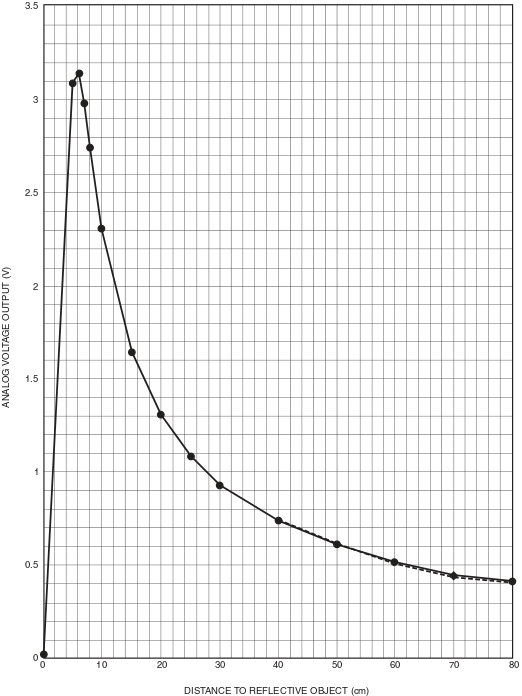
\includegraphics[width=1\textwidth]{figuras/graficair}   
\caption{Gr�fica de tensi�n entre salida para un sensor infrarrojo}
\label{graficair}
\end{figure} 

De esta gr�fica pueden sacarse dos conclusiones. La primera, ya conocida, es que la variaci�n de la salida del sensor y su medida no son proporcionales, por lo que si fuese necesaria extraer medidas en unidades reales habr�a que calcular una adecuaci�n compleja. Sin embargo, esto no ser� necesaria ya que la programaci�n del sensor se basar� en umbrales fijos que ser�n marcados de forma emp�rica. La segunda conclusi�n es que el sensor ofrecer� una tensi�n de salida m�xima de 3.3V. 

La BeagleBone Black dispone de hasta siete entradas anal�gicas como puede observarse en la figura \ref{bbbanal}. Conectaremos las salidas de los dos sensores en dos de estos pines. Sin embargo, consultando el manual de la BeagleBone Black \cite{coley2013beagleboard} observamos que cada entrada anal�gica soporta un m�ximo de 1.8V. Si alimentando el sensor a 5V lo conect�semos directamente, un pico de 3.3V podr�a deteriorar la placa. Por ello, se ha decidido aplicar una simple adecuaci�n de la salida a�adiendo un divisor resistivo. De esta forma, nos cercioraremos de que los 3.3V m�ximos que podr�an salir del sensor se conviertan en 1.8V.

\begin{figure}[H]
\centering
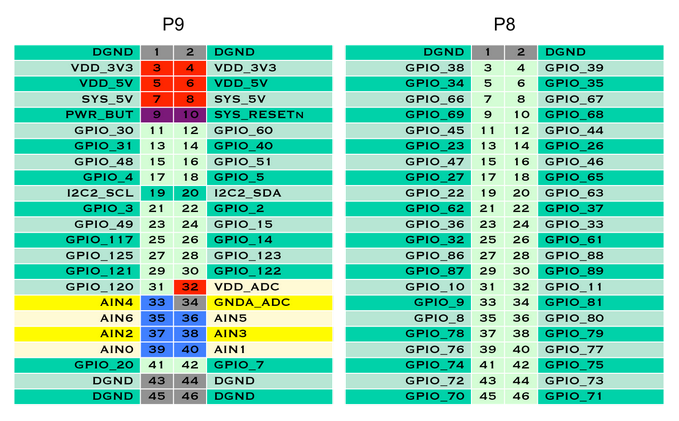
\includegraphics[width=1\textwidth]{figuras/bbbanal}   
\caption{Esquema de entradas anal�gica de una BeagleBone Black}
\label{bbbanal}
\end{figure}

En el esquema de la figura \ref{divir} podemos observar las conexiones que se han realizado entre la placa y el sensor. El sensor es alimentado a 5V a partir del convertidor DC-DC y puesto a tierra com�n con el controlador. La salida del sensor se aplicar� sobre el divisor resistivo, siendo la salida del divisor resistivo la entrada a la BeagleBone Black. Se ha colocado una resistencia de $33k\Omega$ en $Ra$ y una resistencia de $66k\Omega$ en $Rb$.

\begin{figure}[H]
\centering
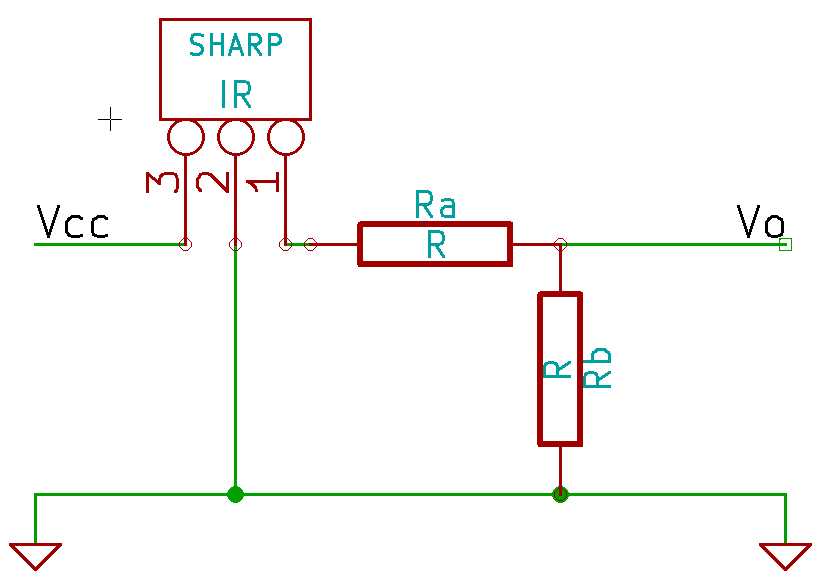
\includegraphics[width=0.65\textwidth]{figuras/divir}   
\caption{Circuito de adecuaci�n de un sensor infrarrojo}
\label{divir}
\end{figure}

\subsection{Br�jula y sensor inercial}

Tanto la br�jula CMPS03 como el sensor inercia MPU9150 han sido conectados por I2C, ambos en el mismo bus. La BeagleBone Black cuenta con dos buses I2C independientes, tal y como se observa en la figura \ref{bbbi2c}.

\begin{figure}[H]
\centering
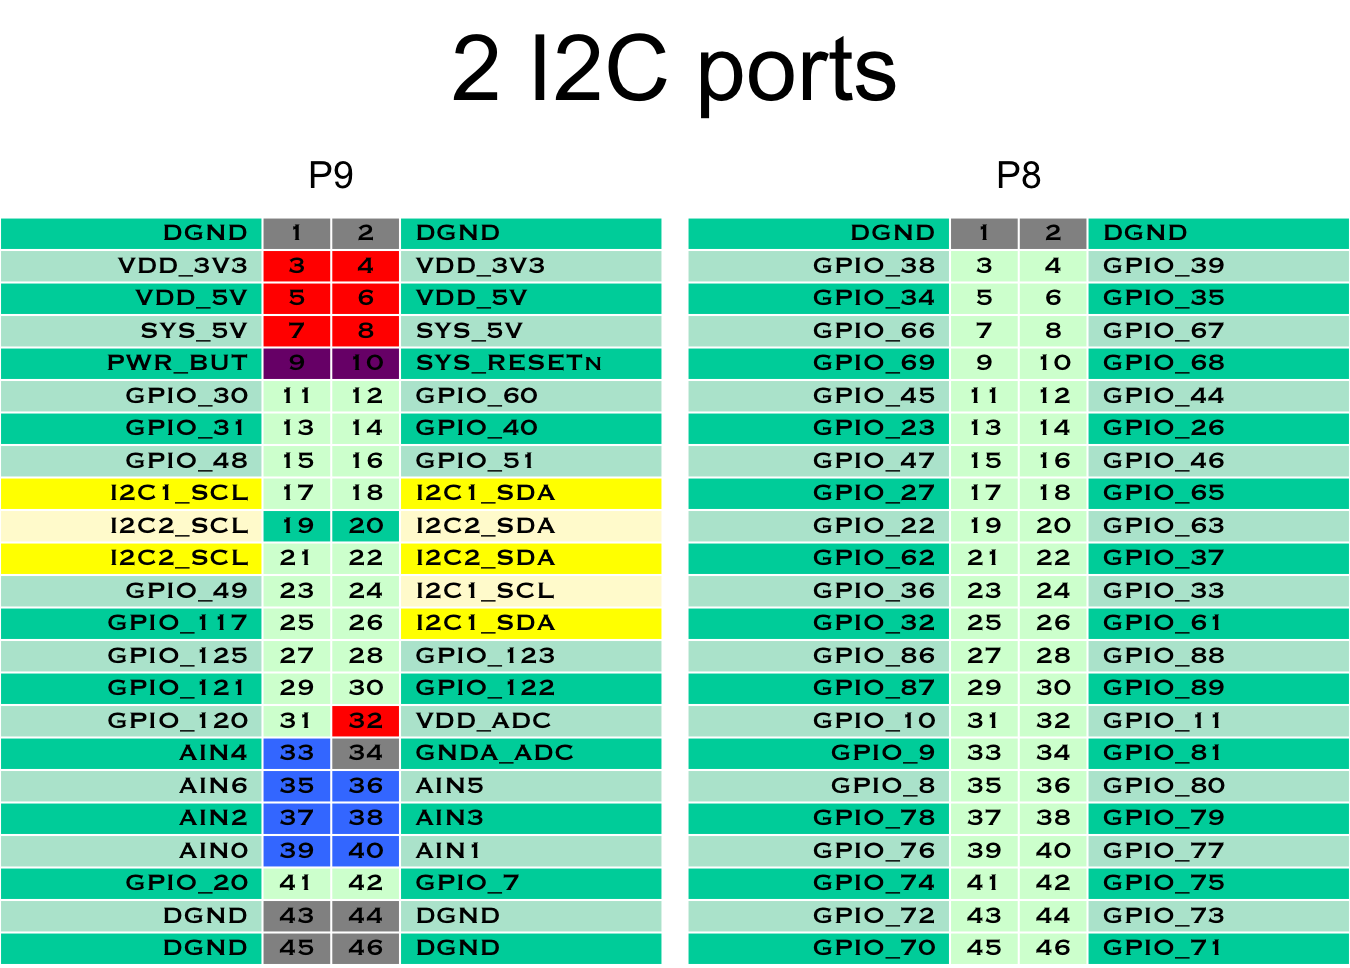
\includegraphics[width=1\textwidth]{figuras/bbbi2c}   
\caption{Esquema de puertos I2C de una BeagleBone Black}
\label{bbbi2c}
\end{figure}

De este modo el sistema ha quedado dise�ado tal y como se muestra en la figura \ref{coni2c}. Cabe destacar que los dos sensores se han alimentado a 3.3V, ya que el MPU9150 los requiere y el CMPS03, aunque se recomienda conectarlo a 5V, funciona perfectamente a 3.3V. Esta tensi�n se ha conseguido desde el pin P9-3 del controlador.

\begin{figure}[H]
\centering
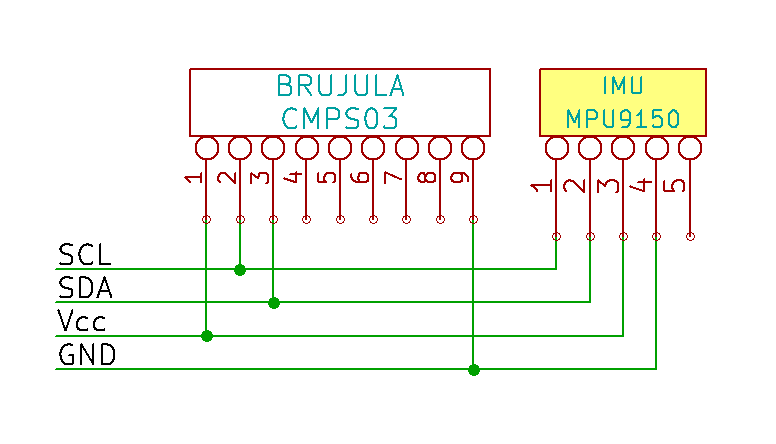
\includegraphics[width=0.85\textwidth]{figuras/esquemai2c}   
\caption{Circuito del bus I2C}
\label{coni2c}
\end{figure} 

\section{Desarrollo de una placa de expansi�n}

Para montar el esquema que se dise�� anteriormente en la figura \ref{dia1} ser� necesario cablear un gran n�mero de conexiones entre dispositivos. Para ello, se ha optado por dise�ar y fabricar una placa de expansi�n que permita conectar todos los dispositivos de una forma limpia y ordenada. Esta placa servir� para comunicar y alimentar las dos placas controladoras, sensores, actuadores y alimentaci�n de todos ellos. El esquema electr�nico puede consultarse en el anexo \ref{anexoesquematico}. A parte, el en anexo \ref{anexofotolitos} se ha inclu�do una copia de los fotolitos de la placa.


\section{Montaje}

Una vez preparados todo los componentes se ha procedido a su montaje. En los siguientes dos apartados se muestra c�mo se ha montado la placa de expasi�n y c�mo se ha integrado la webcam en la cabeza del robot.

\subsection{Montaje de la placa de expansi�n}

La placa de expansi�n ha sido fabricada mediante fresado. Tras enviar los planos a su producci�n se ha obtenido la placa que puede observarse en la figura \ref{montajeplaca1}.

\begin{figure}[h]
\centering
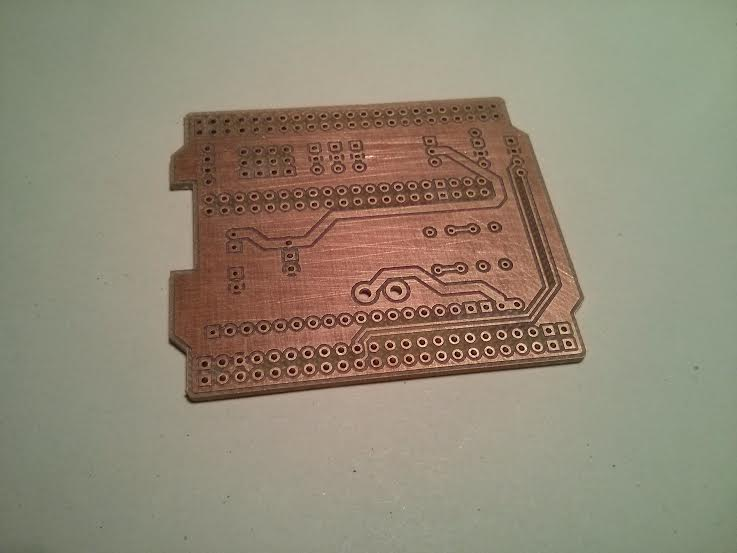
\includegraphics[width=0.5\textwidth]{figuras/montajeplaca1}   
\caption{Placa de expasi�n salida de fabricaci�n}
\label{montajeplaca1}
\end{figure}
\FloatBarrier

Tras esto se ha procedido a soldar todos los componentes que necesita. El listado de los componentes puede consultarse en el anexo TODO. En la im�gen de la figura \ref{montajeplaca2} puede observarse c�mo queda la placa una vez soldada. Adem�s, se le ha realizado un lacado de seguridad con laca aislante. Esto nos ayudar� a evitar posibles accidentes por contacto con conectores y partes met�licas del robot. Finalmente

\begin{figure}[h]
\centering
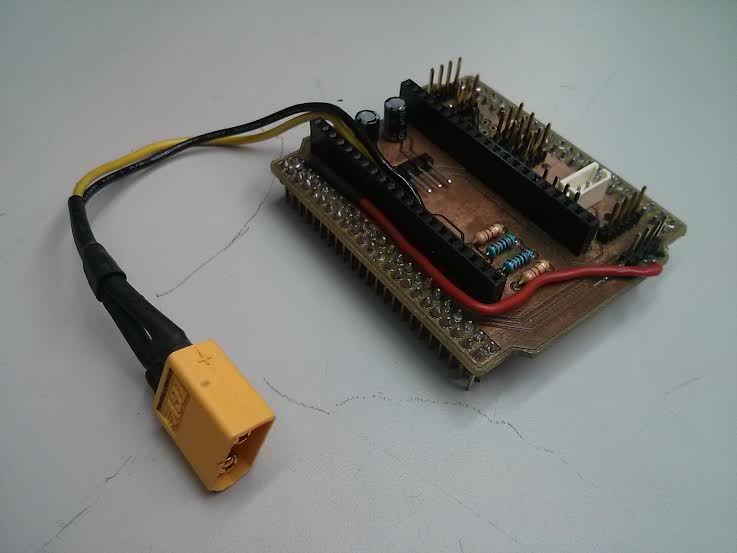
\includegraphics[width=0.5\textwidth]{figuras/montajeplaca2}   
\caption{Placa de expasi�n con componentes soldados}
\label{montajeplaca2}
\end{figure}
\FloatBarrier

\medskip En la figura \ref{montajeplaca3} puede observarse el resultado final del sistema, montado en el robot y conectado a sus componentes.

\begin{figure}[h]
\centering

\includegraphics[width=0.5\textwidth]{figuras/todo}   
\caption{Placa de expansi�n monstada en RAIDER}
\label{montajeplaca3}
\end{figure}
\FloatBarrier


\subsection{Integraci�n de la c�mara en la cabeza}

Para integrar la webcam en la cabeza de RAIDER se ha procedido a desmontar la c�mara Microsoft LifeCam con el objetivo de eliminar su carcasa. El resultado de extraer la c�mara puede observarse en la figura \ref{montajecam1}.

\begin{figure}[h]
\centering
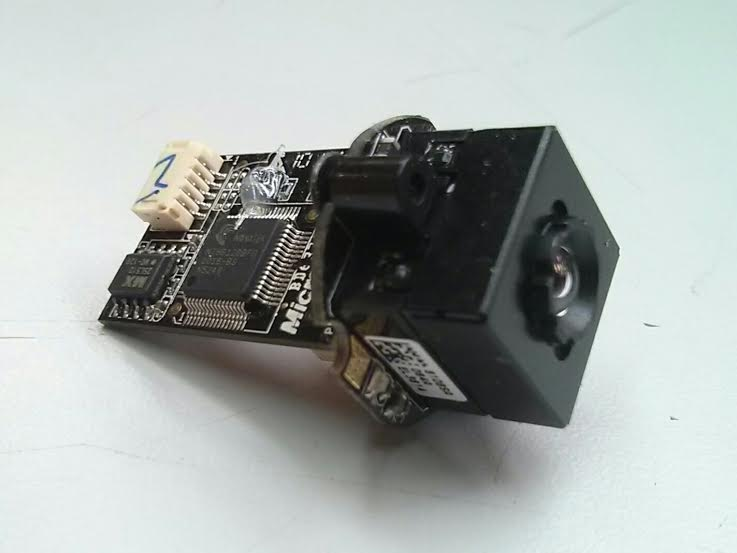
\includegraphics[width=0.5\textwidth]{figuras/montajecam1}   
\caption{C�mara Microsoft LifeCam desmontada}
\label{montajecam1}
\end{figure}
\FloatBarrier

\medskip Ahora, se pasar� a montarla en las piezas imprimibles que se dise�aron para tal efecto. Las piezas aparecen en la figura \ref{montajecam2} junto a la c�mara.

\begin{figure}[h]
\centering
\begin{tabular}{ >{\centering\arraybackslash}m{0.33\textwidth}
>{\centering\arraybackslash}m{0.33\textwidth}
>{\centering\arraybackslash}m{0.33\textwidth}}
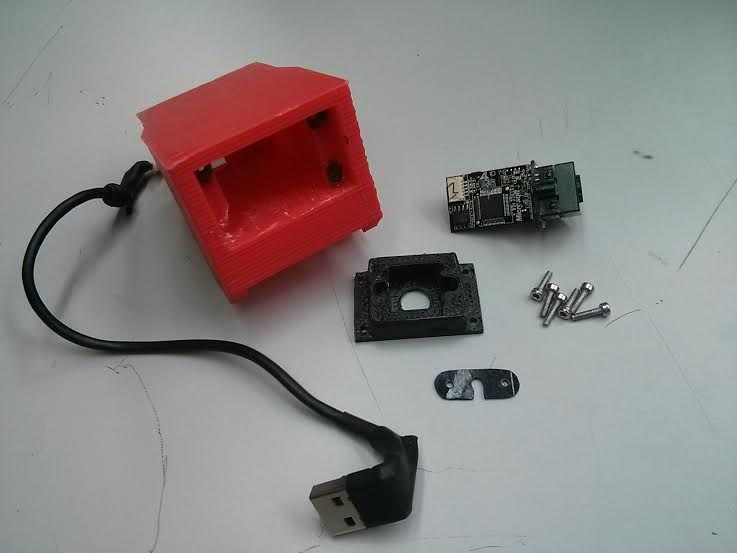
\includegraphics[width=0.33\textwidth]{figuras/montajecam2} &
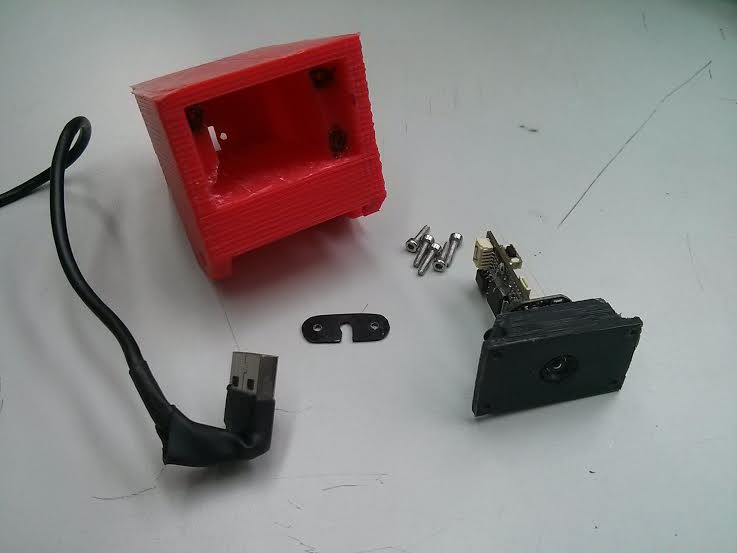
\includegraphics[width=0.33\textwidth]{figuras/montajecam3} &
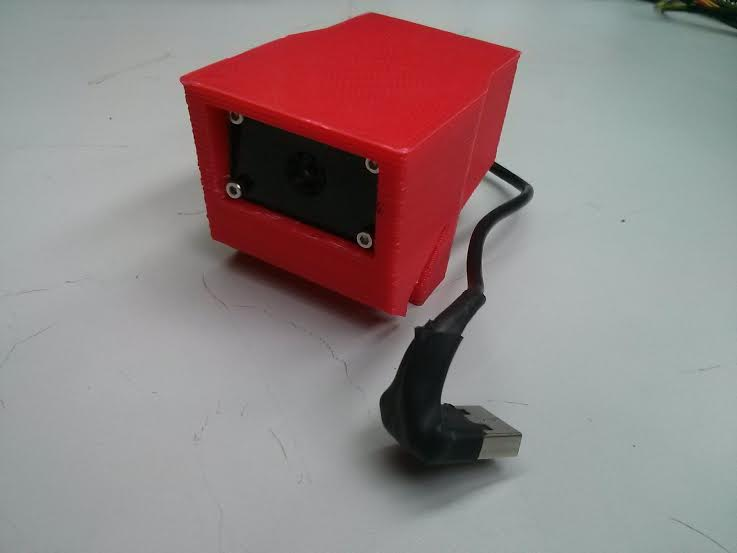
\includegraphics[width=0.33\textwidth]{figuras/montajecam4} \\
\end{tabular}
\caption{Integraci�n de la c�mara en la cabeza}
\label{montajecam2}
\end{figure}
\FloatBarrier

Una vez montado y acortado el cable, procedemos a montar el servo que mover� la cabeza. Como se muestra en la figura \ref{montajecam5}, este se aloja en el cuello.

\begin{figure}[h]
\centering
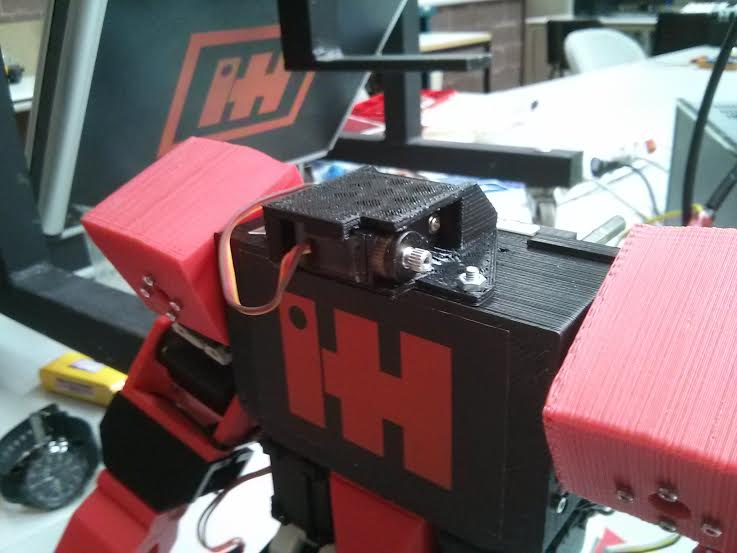
\includegraphics[width=0.47\textwidth]{figuras/montajecam5}   
\caption{Cuello y soporte para la cabeza}
\label{montajecam5}
\end{figure}
\FloatBarrier

Finalmente, en la figura \ref{montajecam6} se muestra el resultado del montaje completo

\begin{figure}[h]
\centering
\begin{tabular}{ >{\centering\arraybackslash}m{0.5\textwidth}
>{\centering\arraybackslash}m{0.5\textwidth}}

\includegraphics[width=0.40\textwidth]{figuras/todo} &

\includegraphics[width=0.40\textwidth]{figuras/todo} \\
\end{tabular}
\caption{Resultado tras la integraci�n de la cabeza en el robot}
\label{montajecam6}
\end{figure}
\FloatBarrier

\subsection{Integraci�n de los sensores infrarrojos en los brazos}

Tal y como se coment� en el apartado TODO, se han integrado dos sensores en los brazos de RAIDER. El motivo de montarlos en los brazos es que se esta manera gozar�n de mayor libertad a la hora de apuntara obst�culos. As� mismo, se ha buscado que el sensor estuviese en una posici�n segura, protegido ante ca�das. En la figura \ref{montajeir1} se pueden observar los dos sensores infrarrojos junto a las piezas que se han dise�ado para alojarlos.

[FOTO de sharps y piezas]
\begin{figure}[h]
\centering
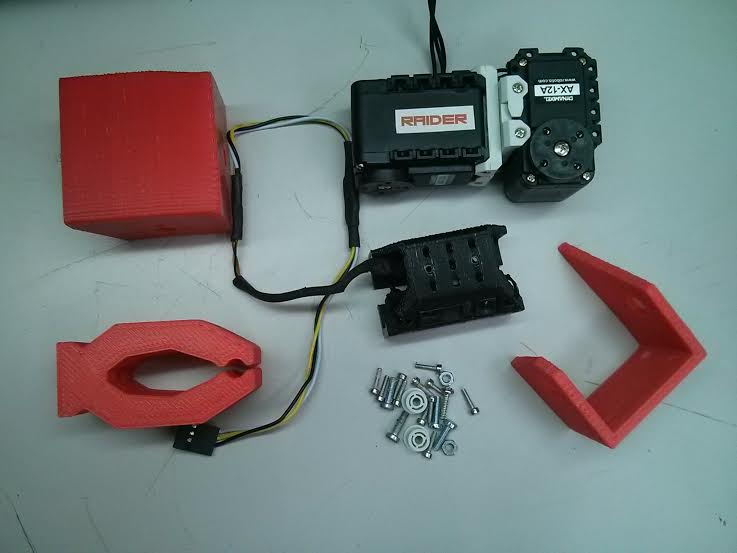
\includegraphics[width=0.5\textwidth]{figuras/montajeir1}   
\caption{Sensores infrarrojos y soportes}
\label{montajeir1}
\end{figure}
\FloatBarrier

Tras montar las piezas, se ha obtenido el resultado mostrado en la figura \ref{montajeir2}

[FOTO del conjunto]
\begin{figure}[H]
\centering

\includegraphics[width=0.5\textwidth]{figuras/todo}   
\caption{Brazos con sensores montados}
\label{montajeir2}
\end{figure}
\FloatBarrier


  
  %partes finales del trabajo: conclusiones, bibliografia y anexos
\backmatter

\chapter{Evaluaci�n de resultados}

En este cap�tulo se presentar�n las conclusiones y consideraciones que se han podido extraer de este proyecto.

\section{Pruebas }

Llegados a este momento, RAIDER ha sido montado y puesto en marcha. Se han desarrollado aplicaciones sobre el robot que le han permitido asistir a diferentes competiciones y exhibiciones.

\medskip En Spain Experience, se puso a prueba la resistencia y autonom�a de la plataforma. Durante mas de dos horas, el robot se control� de forma remota sobre el campo de juego. Durante la exhibici�n tuvo que dar patadas a un bal�n, correr al lado de otros robots (algunos de una categor�a superior a los mini-humanoides), reincorporarse despues de algunas ca�das y en definitiva, aguantar con una misma bater�a hasta diez minutos de uso.

\medskip Los resultados fueron muy satisfactorios. Las piezas imprimibles aguantaron los golpes que recibi� en robot durante su operaci�n y el sistema electr�nico no sufri� ning�n tipo de calentamiento o de interrupci�n en su funcionamiento.

\medskip Por otra parte, RAIDER se present� a tres pruebas del campeonato CEABOT. En la modalidad de visi�n, fue el �nico robot capaz de diferenciar m�s de un marcador, llegando a la cifra de cuatro marcadores detectados y ejecutados correctamente. Esta actuaci�n supuso el primer puesto de la prueba de visi�n.

\medskip En la prueba de navegaci�n, el robot fue capaz de superar la prueba completa en un tiempo de dos minutos y trece segundos, siendo el �nico robot capaz de realizar el camino de vuelta desde la zona de llegada parcial. Esta marca se tradujo en el primer puesto en la prueba de navegaci�n.

\medskip Por �ltimo, la prueba de sumo cont� con siete robots participantes. Tras varios combates, RAIDER escal� en la clasificaci�n hasta la final, pero fue vencido en el �ltimo duelo. Sin embargo, consigui� el segundo puesto de la prueba de sumo.

\medskip Tras estas tres prueba, RAIDER qued� en el segundo puesto de la clasificaci�n global, a�n contando con el handicap de no haber participado en la prueba de escaleras.

\section{Conclusi�n}

Una vez finalizado el proyecto, las impresiones han sido muy positivas. Considero que los objetivos propuestos se han alcanzado con un alto grado de satisfacci�n. RAIDER ha demostrado ser un robot con unas capacidades muy aptas para la competici�n y la investigaci�n. 

\medskip A parte de ello, dejando de lado el robot, pienso que este trabajo me ha aportado conocimientos en diferentes �reas de la ingenier�a que no podr�a haber conseguido de otro modo.

\section{Desarrollos futuros}

El t�rmino de este proyecto supone un punto de partida para nuevos desarrollos basados en la plataforma rob�tica mini-humanoide RAIDER. Por una parte, se propone la mejora de las capacidades de desplazamiento bipedo. En su estado actual, el robot tiene la capacidad suficiente para realizar controles de estabilidad avanzados, gracias a sus sensores inerciales y a la informaci�n que ofrecen los servomotores escogidos.

\medskip Por otra parte, se prevee una mejora a nivel mec�nico incluyendo piezas de fibra de carbono y aumentando el n�mero de grados de libertad del robot con servos de mayor potencia.

\medskip Tambi�n, el que seguramente sea el paso inmediatamente posterior, se integr�n manipuladores en las extremidades del robot. Unas manos m�viles aportar�n una mayor capacidad de interacci�n con el entorno, y podr�n programarse algoritmos de grasping. Los pies tambi�n suponen un punto importante a la hora de realizar mejoras. Unos pies con sensores ser�an my �tiles a la hora de controlar mejor la marcha b�peda y tambi�n para realizar tareas como la de subir y bajar escaleras.

\medskip Al mismo tiempo, se seguir�n realizando algoritmos de visi�n sobre la BeagleBone Black, una placa que ha demostrado tener unas capacidades muy interesantes para su montaje en peque�os robots. Adicionalmnte, se prevee una reutilizaci�n de las librer�as desarrolladas durante el proyecto para su aplicaci�n en otros sistemas.

%estilo de bibliograf�a: plana, alfa...
\bibliographystyle{plain}

%genera doble hoja en blanco
\cleardoublepage

%apartado de bibliograf�a
\addcontentsline{toc}{chapter}{Bibliograf�a}

%se incluye la bibliograf�a. Archivo de tipo .bib (bibtex)
\bibliography{bibliografia}

%fin del documento
\end{document}